
% Created 2011-10-27 do 16:51
\documentclass[a4paper, 10pt]{article}
\usepackage[utf8]{inputenc}
\usepackage[T1]{fontenc}
\usepackage{fixltx2e}
\usepackage{graphicx}
\usepackage{longtable}
\usepackage{float}
\usepackage{wrapfig}
\usepackage{soul}
\usepackage{textcomp}
%\usepackage{marvosym}
%\usepackage{wasysym}
%\usepackage{latexsym}
%\usepackage{amssymb}
\usepackage{mathtools}
\usepackage{hyperref}
\usepackage{placeins}
\usepackage{pict2e}
\usepackage{subfig}
%\usepackage{cmbright}
\usepackage[dutch]{babel}
\usepackage[a4paper,margin=2.5cm]{geometry}
 \hyphenpenalty=5000
\tolerance=1000
\providecommand{\alert}[1]{\textbf{#1}}
\newfloat{MATLAB code}{h}{}
\usepackage{tikz,pgfplots}

\pgfplotsset{compat=newest}
\pgfplotsset{plot coordinates/math parser=false}

\title{Thesisverslag 1}
\author{Roel Matthysen - \today}
\date{}

\newlength\figureheight
\newlength\figurewidth
\setlength\figureheight{2cm}
\setlength\figurewidth{12cm}


\begin{document}

\maketitle

\section{Activiteiten}
\begin{description}
\item[Literatuur] \hfill\begin{itemize} Leesbare scans van alle formules uit het artikel (bibliotheek).\end{itemize}
\item[MATLAB] \hfill\begin{itemize}
\item Voorlopige implementatie van de algoritmes 1, 2 en 3. De algoritmes zijn ge\"implementeerd met MATLAB-indexering voor arrays (1:n) om de correctheid van de algoritmes gemakkelijker na te kunnen gaan.
\item Testen met de s-dimensionele $\prod_{j=1}^s B_2(x_j)$ veelterm, voor $s=2..10$.
\end{itemize}
\end{description}
\section{resultaten}
De resultaten als de kwadratische fout voor $2^n$ punten (n=2..12) wordt getoond in figuur \ref{fig:korobov3algorithms} voor verschillende dimensies. De fout wordt getoond voor de drie algoritmes, en voor een Sobol puntenset (geen scramble of shift)  ter vergelijking. De punten verkregen met de Korobov algoritmes geven een fout vergelijkbaar met die verkregen uit een Sobol set. 

\subsection{Opmerkingen}
\emph{Dit probleem is verholpen en lag aan een foute communicatie tussen de verschillende methodes.}

\hfill\newline
\noindent Bij dimensie 2 en 4 punten geven alle drie de algoritmes een resultaat dat gespiegeld is tov de resultaten van de Sobol set, maar nog steeds correct, met (0.25,0.25) als generator, als in figuur \ref{fig:2dimensions4points}. Bij algoritmes 1 en 3  geeft een groter aantal punten dan een juist resultaat (figuur \ref{fig:2dimensions8points1}), maar bij algoritme 2 is voor twee dimensies de generator altijd een eenheidsvector (figuur \ref{fig:2dimensions8points2}). Dit doet vermoeden dat er nog een fout zit in de implementatie van algoritme 2.

\section{Verder werk}
\begin{itemize}
\item Testen met een andere testfunctie
\item Nadenken over een effici\"entere implementatie, om uiteindelijk tot de ordes uit het artikel te komen. In de MATLAB implementatie zijn daarvoor nog te veel lussen gebruikt.
\item Nakijken waar eventuele numerieke fouten zich zouden kunnen voordoen, omdat er vaak gedeeld wordt door grote getallen.
\end{itemize}

\begin{figure}[htp]
\centering

\includegraphics{img/2dimensions4points.eps}
\caption{Situatie wanneer $s=2$ en \# punten = 4.}
\label{fig:2dimensions4points}
\end{figure}
\begin{figure}[htp]
\centering
\subfloat[Algoritme 1,3]
{
\includegraphics{img/2dimensions8points1.eps}\label{fig:2dimensions8points1}}
\subfloat[Algoritme 2]
{
\includegraphics{img/2dimensions8points2.eps}\label{fig:2dimensions8points2}}
\caption{Situatie bij $s=2$ en \# punten = 8}
\label{fig:}
\end{figure}

\begin{figure}[htp]
\centering
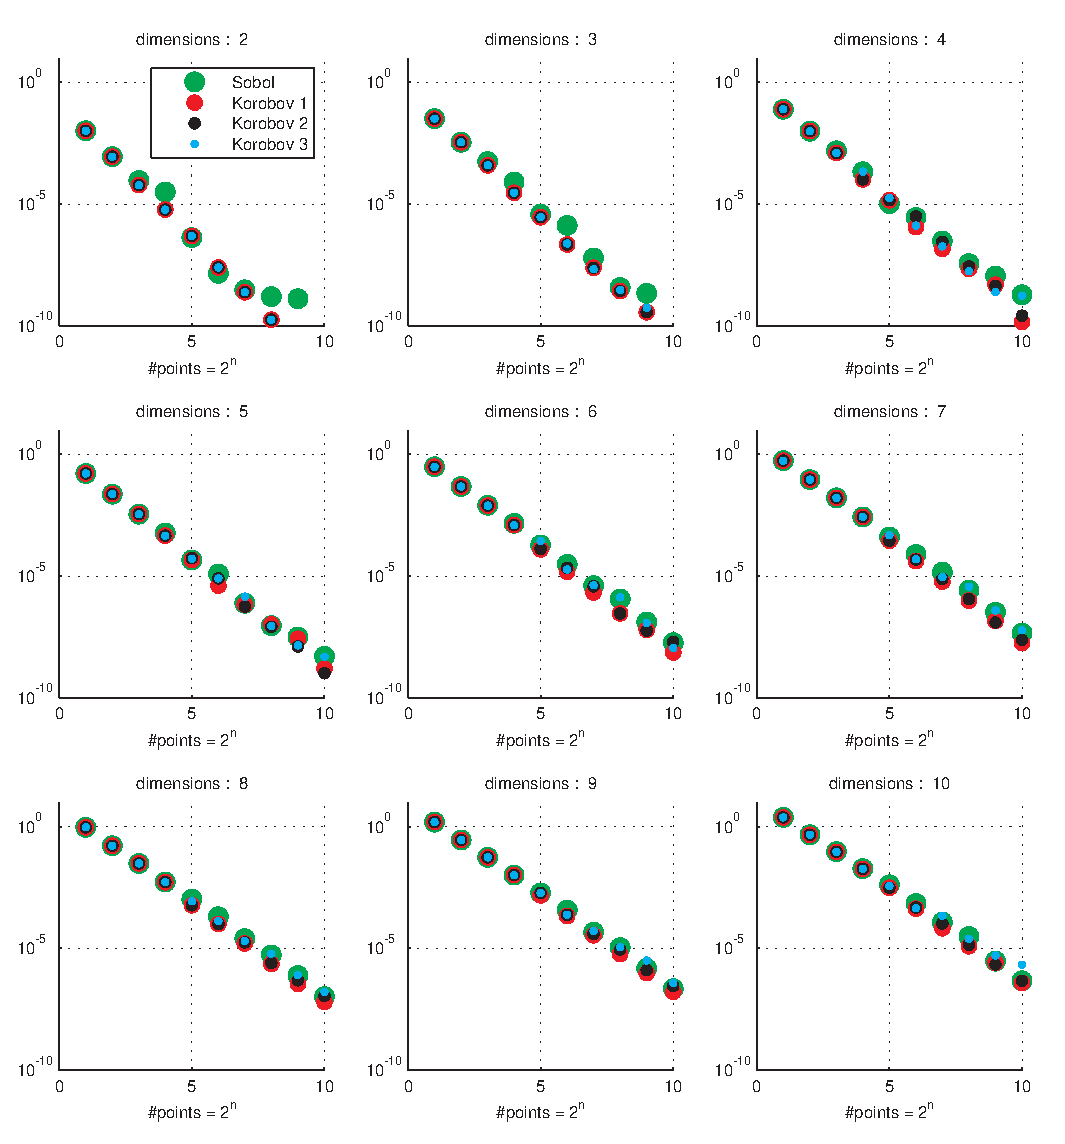
\includegraphics{img/korobov3algorithms.eps}
\caption{De kwadratische fout voor de testfunctie $B_2$ in verschillende dimensies.}
\label{fig:korobov3algorithms}
\end{figure}




\end{document}

%%% Local Variables: 
%%% mode: latex
%%% TeX-master: t
%%% End: